% !TEX root =  main.tex
\newpage
\chapter{Application design} \label{ch:sw_design}
The VPP application is implemented in object-oriented Python. The static structure and runtime behavior is det

\section{Static structure}

\begin{figure}[H]
    \centering
    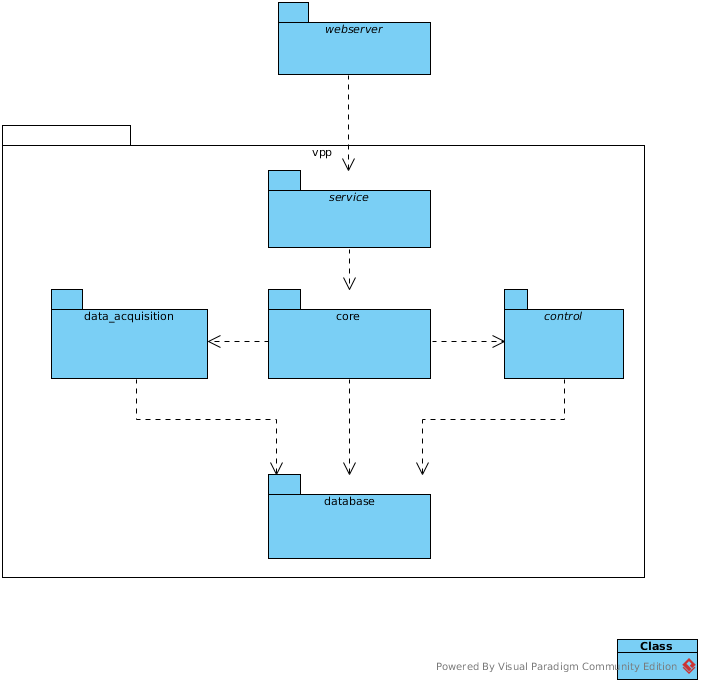
\includegraphics[width=0.5\textwidth]{figures/class_overview}
    \caption{Package diagram}
    \label{figureClassDiagram}
\end{figure}

The application is roughly structured in a layered architecture with the \texttt{database} as the bottom layer and the \texttt{core} and \texttt{data\_acquisition} packages as the domain layer. A \texttt{service} package could be added as the top layer, providing an external interface. The packages are explained in detail below.


\subsubsection{Package \texttt{vpp.core}}

\begin{figure}[H]
    \centering
    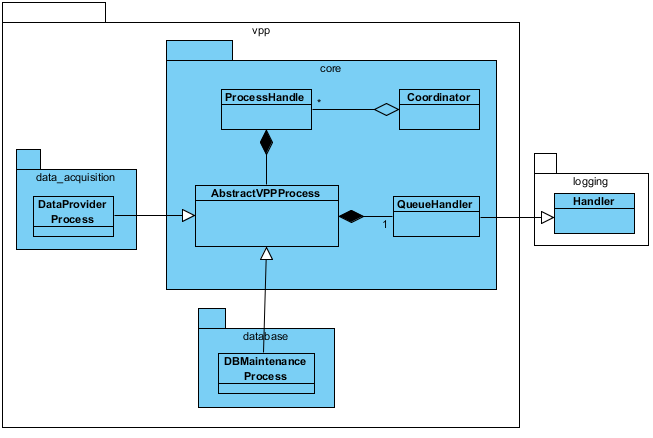
\includegraphics[width=\textwidth]{figures/class_core}
    \caption{Core}
\end{figure}

\texttt{Coordinator} is called by \texttt{start\_server.sh} and launches the entire application. Mainly, it instantiates the \texttt{DataProviderProcess} and the \texttt{DBMaintenanceProcess}. The processes are each wrapped in a \texttt{ProcessHandle} which handles process launch and termination and receives log messages from the underlying process.


\subsubsection{Package \texttt{vpp.data\_acquisition}}

\begin{figure}[H]
    \centering
    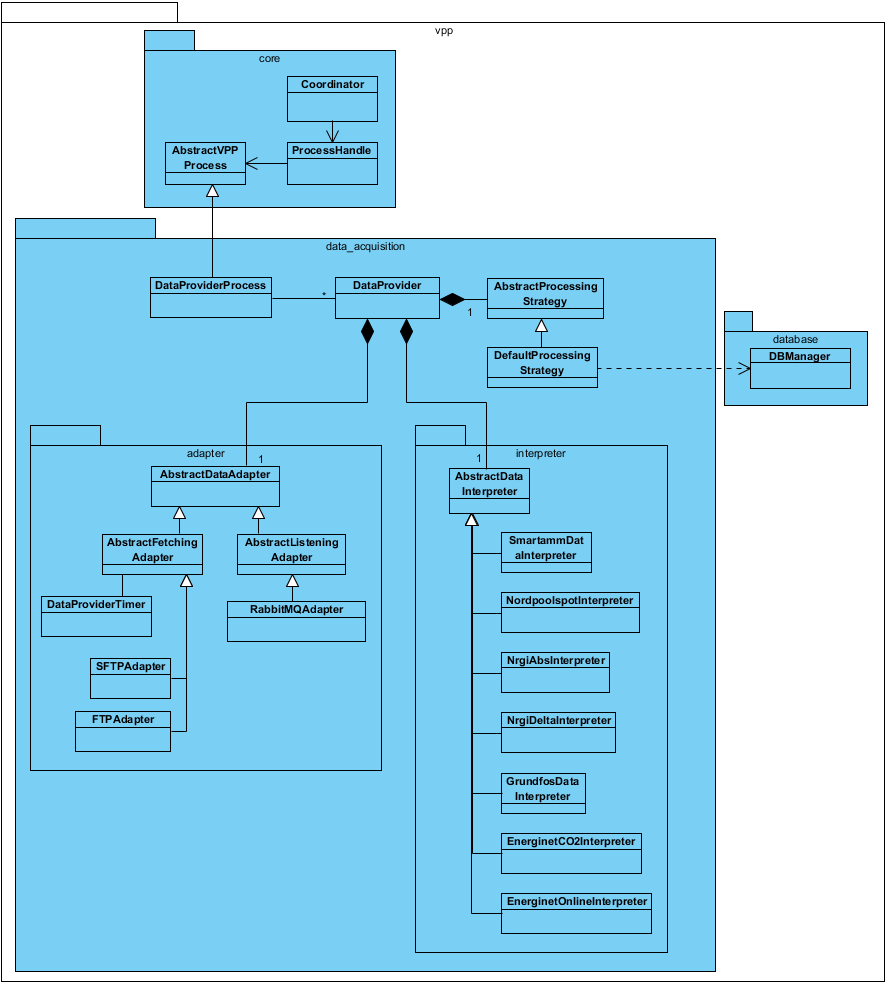
\includegraphics[width=\textwidth]{figures/class_data_acquisition}
    \caption{Data acquisition}
\end{figure}

This package contains the framework for connecting to sources of measurement and prediction data. The \texttt{DataProviderProcess} launches a \texttt{DataProvider} for each configured \texttt{.ini}-file as described in \ref{sec:data_provider_config}. Each \texttt{DataProvider} instance employs a suitable \texttt{DataAdapter}. The \texttt{FetchingAdapter}s employ a \texttt{DataProviderTimer} that will wake up according to configuration and execute data retrieval and processing. The \texttt{ListeningAdapter} will launch a thread that continuously listens for messages and processes them as they are received. Thus, each data provider does all processing in its own thread.

The \texttt{DataAdapters} handle communication with the data source and extract a raw string that is then passed to the configured \texttt{DataInterpreter}. The interpreter parses the string and outputs data as Python dictionaries to the \texttt{ProcessingStrategy} which interacts with a \texttt{DBManager} to store the data.


\subsubsection{Package \texttt{vpp.database}}

This package contains the code that interfaces directly with the database. 

\begin{figure}[H]
	\centering
	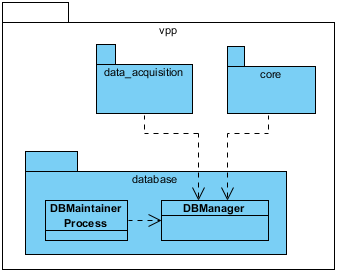
\includegraphics[width=0.5\textwidth]{figures/class_db}
	\caption{Database TODO update figure}
	\label{}
\end{figure}

\texttt{DBMaintainer} will run maintenance on the database and implement the Rolling Window strategy.

Communication with the database could be implemented simply using SQL, or we could opt for an object-relational mapper (ORM) framework such as SQLAlchemy.


\section{Runtime processes}

Separate Python processes are deployed to enable concurrent processing. Using processes instead of threads is necessary to fully utilize multiple cores, since Python employs a \emph{Global Interpreter Lock} which prevents threads within the same Python interpreter from executing concurrently. Using processes mitigates this as each process will run with its own interpreter. For this prototype, the multiprocessing could probably have been omitted in favor of simpler multithreading since CPU load has not been an issue at all.

The runtime creation of processes within the main server application is shown below:
\begin{figure}[H]
    \centering
    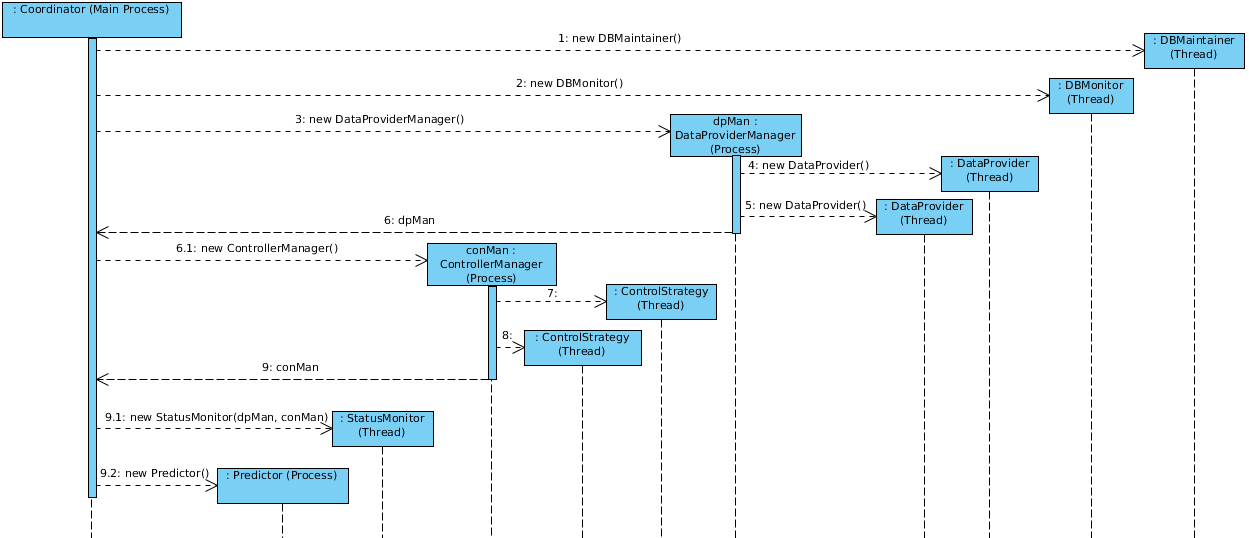
\includegraphics[width=\textwidth]{figures/seq_diagram}
    \caption{Sequence diagram of thread creation}
    \label{figureSeqDiagram}
\end{figure}
As can be seen, at least six concurrent processes will be running in addition to any \texttt{DataProviders} configured.


\subsubsection{Process communication overhead}
There is of course an overhead cost involved in running processes as opposed to threads, since processes do not have shared memory which will make communication more costly performance-wise. A balanced approach could be to group processes with frequent communication as threads within the same process, thus reducing the total number of processes form the current minimum six (plus \texttt{DataProviders}) to two or three. 

\subsection{Logging - interprocess}

\newpage
\subsection{Data acquisition}
The execution flow when receiving measurements from a RabbitMQ is shown below:
\begin{figure}[H]
    \centering
    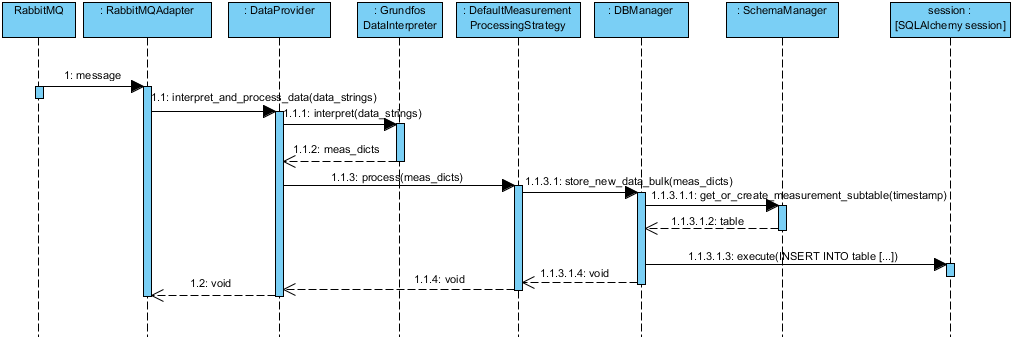
\includegraphics[width=\textwidth]{figures/data_acq_seq_diagram}
    \caption{Sequence diagram of data acquisition}
    \label{figureSeqDiagram}
\end{figure}


\subsection{Web server}\label{subsection:webserver}
We intend to provide a web interface for users to access the system. This will run in a separate web server, but in the same machine. The preliminary plan is to build the webapp using Django since this supports Python. 

The web interface could in itself grow to a rather large application with support for building configuration, device configuration, user administration, actuation interfaces and so on. This will require a substantial design and development effort. In the initial version, we plan to support only very basic interaction as proof of concept.